Figure \ref{fig:sensing} outlines the on-board sensing capabilities that will be available to the aircraft. Each sensor is detailed below.

\begin{figure}[!h]
	\centering
	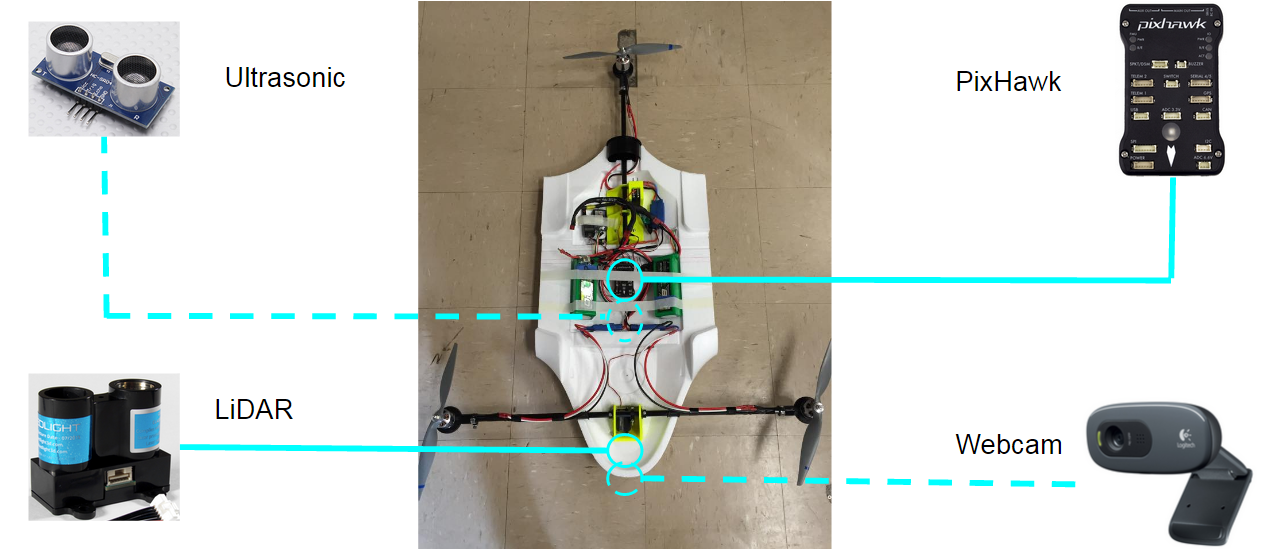
\includegraphics[width=300pt]{Images/sensors}
	\caption{Onboard sensing capabilities}
	\label{fig:sensing}
\end{figure}

\subsubsection*{PixHawk Flight Controller}
The PixHawk has several in-built or plug-and-play sensors, including a 3-axis accelerometer, altimeter, compass, and GPS. The PixHawk will provide the aircraft's telemetry to the main processor, which will be augmented by the additional sensors below.

\subsubsection*{Ultrasonic Module}
The ultrasonic module will be mounted underneath the aircraft. It will provide a more reliable and controllable height measurement than the PixHawk's inbuilt altimeter, and will assist in the aircraft's autonomous landing.

\subsubsection*{Webcam}
The webcam will mounted beneath the nose of the aircraft. It will provide vision for the aircraft's obstacle avoidance maneuvers, and will form the basis for identifying Joe's blue jeans.

\subsubsection*{LiDAR}
The LiDAR will be mounted in the nose of the aircraft. The LiDAR can only measure the range of objects directly in front of it, so it will be mounted on a dual servo system that allows it to sweep a hemisphere in front of the aircraft (see Figure ). It will provide a 3D map of the environment in front of the aircraft, and will assist in path planning and obstacle avoidance.

\begin{figure}[!h]
	\centering
	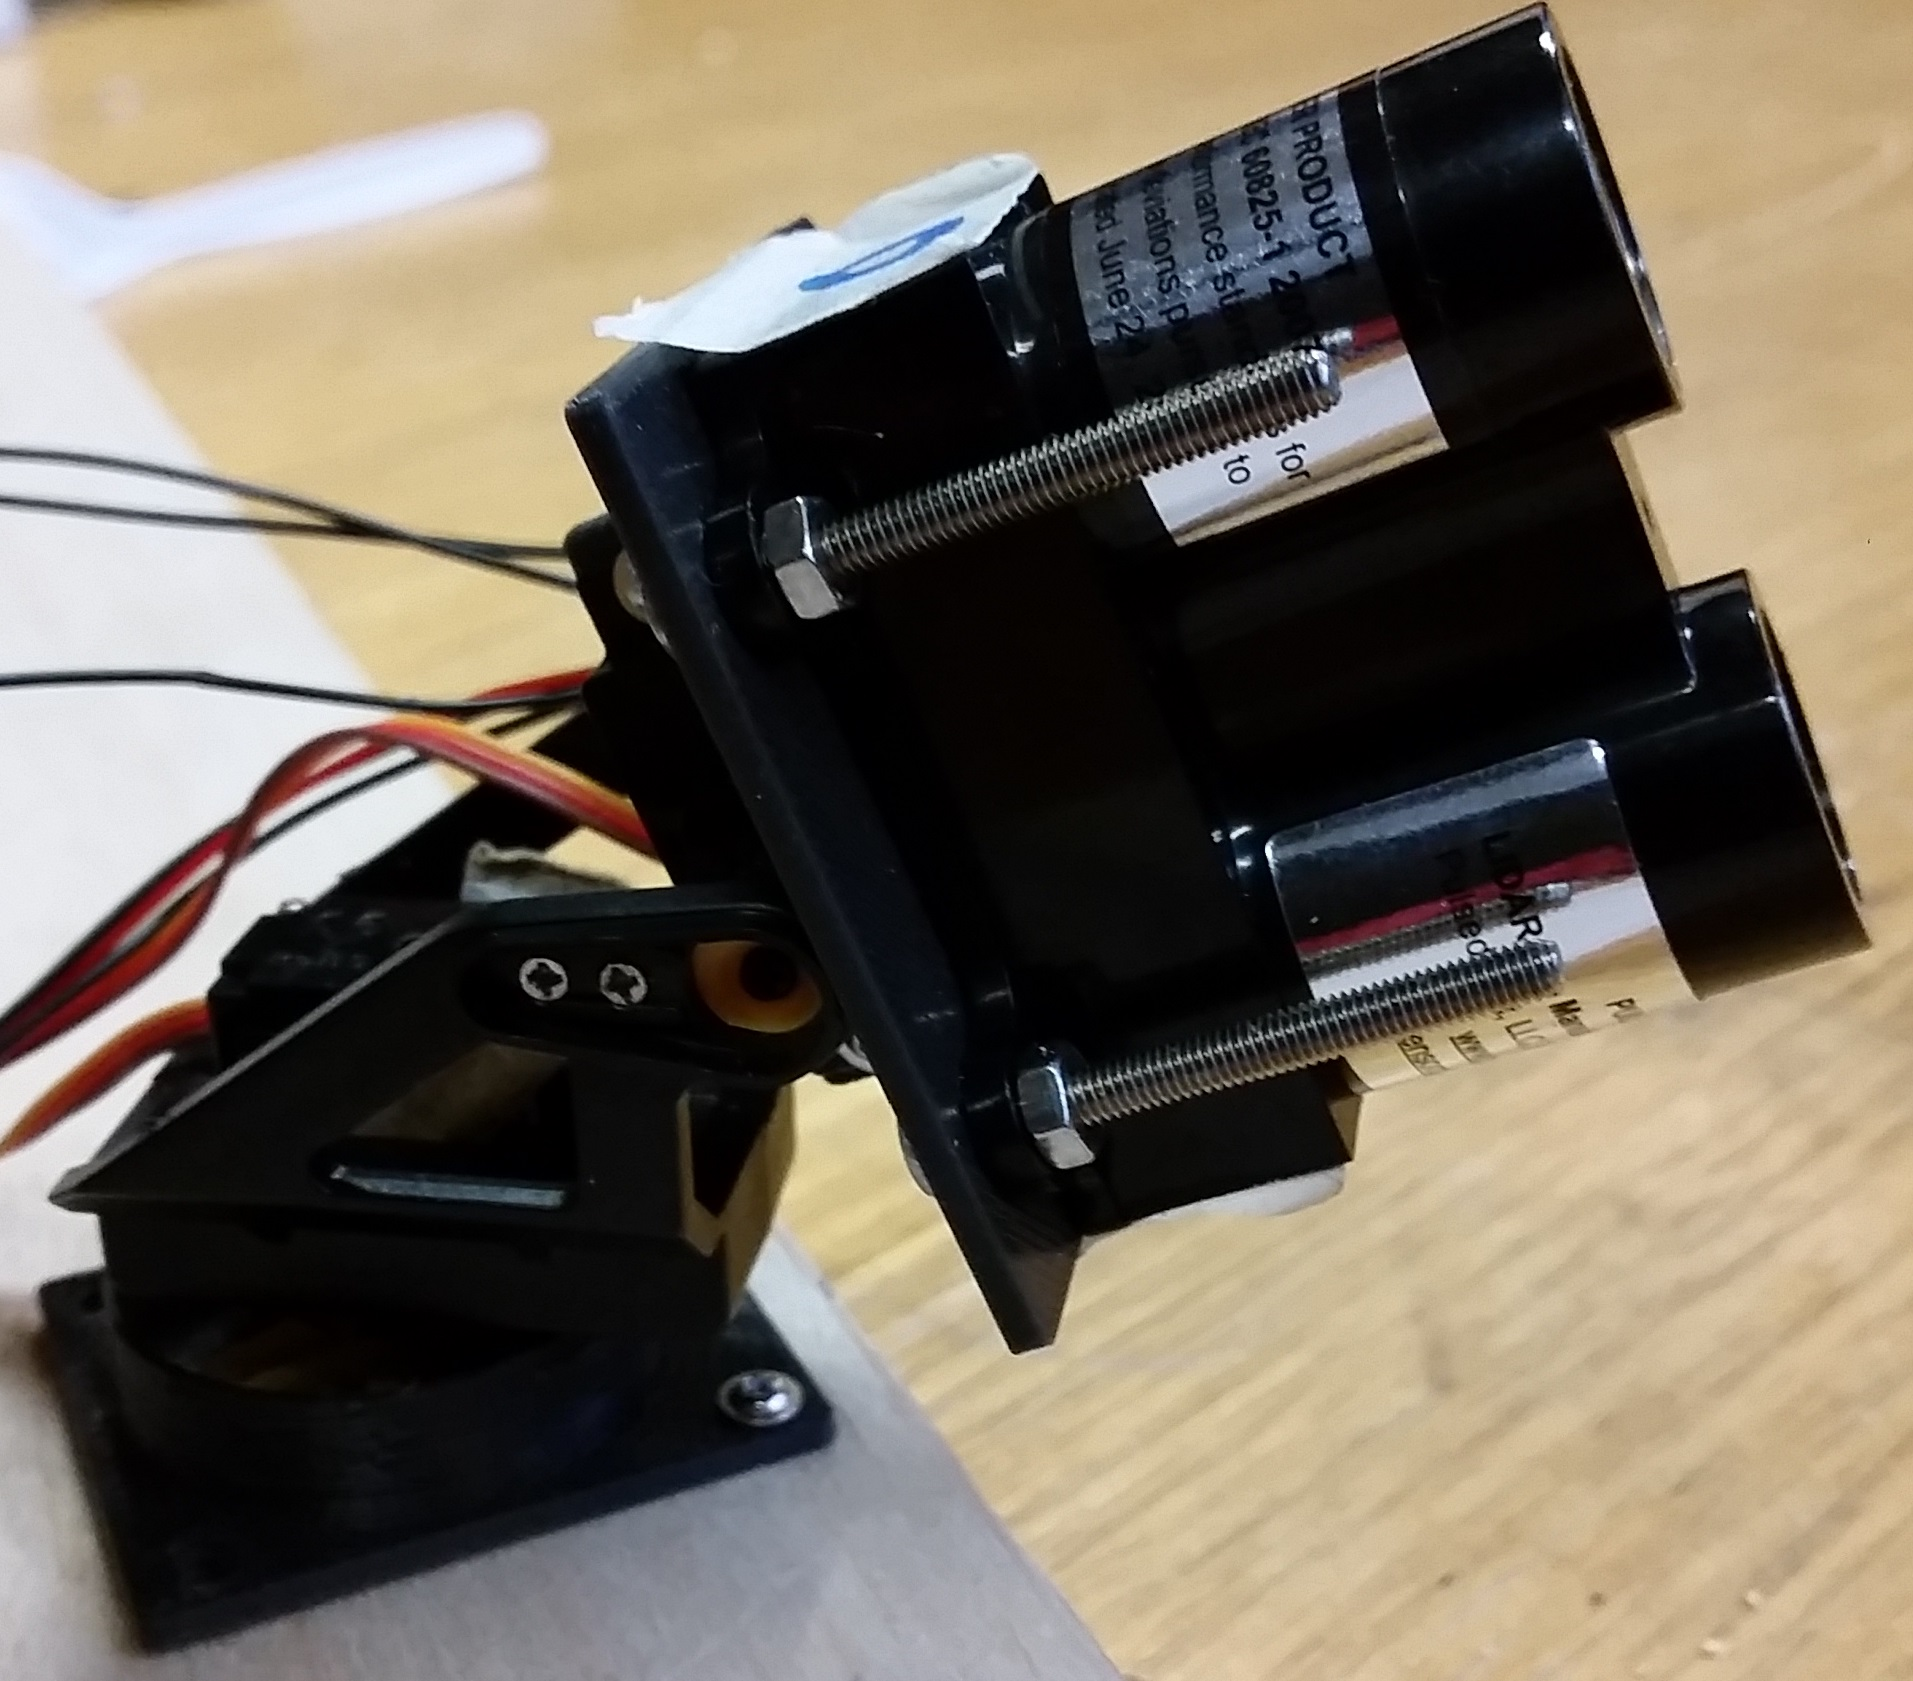
\includegraphics[width=100pt]{Images/lidar}
	\caption{LiDAR mounting}
	\label{fig:lidar}
\end{figure}